\documentclass[11pt,a4paper]{article}
\usepackage[T1]{fontenc}
\usepackage[utf8]{inputenc}
\usepackage{lmodern}
\usepackage[margin=2.4cm]{geometry}
\usepackage{amsmath,amssymb}
\usepackage{graphicx}
\usepackage{booktabs}
\usepackage{siunitx}
\usepackage[font=small,labelfont=bf]{caption}
\usepackage{microtype}
\usepackage[hidelinks]{hyperref}
\usepackage{xcolor}
\usepackage{fancyhdr}
\usepackage{enumitem}

\sisetup{detect-all,per-mode=symbol}
\definecolor{navy}{HTML}{1F4E79}
\definecolor{brick}{HTML}{C0392B}
\newcommand{\pending}[1]{\textcolor{brick}{\textbf{[PENDING]} #1}}
\newcommand{\verifyc}{\textcolor{brick}{\footnotesize[verify]}}

\pagestyle{fancy}\fancyhf{}
\lhead{\footnotesize Wettability-dependent bubble-coverage closure for AWE}
\rhead{\footnotesize \thepage}
\renewcommand{\headrulewidth}{0.3pt}

\title{\bfseries A wettability-dependent bubble-coverage closure for open-source
alkaline water electrolyser CFD, derived from potential-aware molecular dynamics
and interface-resolved simulation}

\author{[TO BE COMPLETED]\\[2pt]
\normalsize Affiliations: [TO BE COMPLETED]\\
\normalsize Corresponding author: [TO BE COMPLETED]}
\date{Draft --- \today}

\begin{document}
\maketitle

\begin{center}
\fbox{\begin{minipage}{0.93\textwidth}\small
\textbf{Draft status.} Sections~\ref{sec:intro}--\ref{sec:methods} (Introduction, Theory,
Methods) are drafted. Section~\ref{sec:results} reports \emph{only} the force-field validation
results, which exist; every other subsection is a structural placeholder marked \pending{}.
The simulation campaign is in progress. \textbf{No number in this manuscript is unsupported by a
file in the project repository.} Target journal: \emph{International Journal of Hydrogen Energy}.
\end{minipage}}
\end{center}

\section*{Abstract}
\pending{To be written once the closure exists. Structure fixed in advance so it cannot be
retrofitted: (i) coverage closures used in alkaline water electrolyser CFD are empirical
correlations fitted at low current density; (ii) we derive the wettability dependence of coverage
from constant-potential molecular dynamics and interface-resolved simulation; (iii) the resulting
effect on predicted cell polarisation relative to the legacy closure; (iv) the validity envelope of
the derived closure.}

\vspace{4pt}\noindent\textbf{Keywords:} alkaline water electrolysis; bubble coverage; wettability;
contact angle; constant-potential molecular dynamics; volume of fluid; OpenFOAM; multiscale modelling

%==========================================================================
\section{Introduction}\label{sec:intro}

\subsection{Bubble coverage is the dominant closure in alkaline electrolyser models}

Alkaline water electrolysis (AWE) is the most mature route to large-scale hydrogen production, and
its efficiency at industrially relevant current density is limited in large part by the bubbles it
generates. Hydrogen evolves at the cathode and oxygen at the anode as discrete bubbles that
nucleate, grow, adhere, and eventually detach. While attached, a bubble blanks off catalytically
active area and displaces conductive electrolyte. The blanked fraction---the bubble coverage
$\Theta$---degrades performance through three distinct routes: reduced active area for charge
transfer, reduced effective electrolyte conductivity, and obstructed species transport.

The activation penalty is the most direct. If a fraction $\Theta$ of the electrode is screened, the
same total current passes through the remainder, so the local current density rises to
$j/(1-\Theta)$. In the Tafel limit this costs
\begin{equation}
\Delta\eta_{\mathrm{act}} = \frac{RT}{\alpha n F}\,\ln\!\left(\frac{1}{1-\Theta}\right)
\label{eq:tafel}
\end{equation}
At $\alpha=0.5$, $n=1$ and \SI{353}{\kelvin} the prefactor $RT/(\alpha nF)$ is \SI{60.84}{\milli\volt},
so $\Theta=0.2$ costs \SI{13.6}{\milli\volt} while $\Theta=0.8$ costs \SI{97.9}{\milli\volt}. The
penalty is strongly non-linear in $\Theta$, which is why an error in the closure matters
disproportionately at high current density.

\paragraph{Kinetic convention.} Equation~\eqref{eq:tafel} carries $n$ explicitly. This work assumes
a Volmer-limited cathodic reaction with a one-electron rate-determining step,
$\alpha_{\mathrm{app}}=\alpha n = 0.5$, implying a Tafel slope of
\SI{140.1}{\milli\volt\per dec} at \SI{353}{\kelvin}. This is stated because the choice matters: were
the Heyrovsky step rate-determining ($\alpha_{\mathrm{app}}\approx 1.5$,
\SI{46.7}{\milli\volt\per dec}), the same coverage would cost only \SI{32.7}{\milli\volt}. The
headline quantity of this study depends on the assumed elementary step by a factor of three, and
both values are reported.

\subsection{The closure in use was fitted far below where it is applied}

Cell-scale AWE models close $\Theta$ with empirical correlations, overwhelmingly of the form
introduced by Vogt and co-workers. Vogt and Balzer~\cite{vogt2005} give
\begin{equation}
\Theta = \left(\frac{j}{3\times10^{5}\ \mathrm{A\,m^{-2}}}\right)^{0.3}
       = 0.023\left(\frac{j}{\mathrm{A\,m^{-2}}}\right)^{0.3}
\label{eq:vogt}
\end{equation}
for stagnant electrolyte, and Eigeldinger and Vogt~\cite{eigeldinger2000} supply the flow correction
\begin{equation}
\Theta = \frac{\Theta_0}{\left[1+(C_4 v)^2\right]^2}, \qquad C_4 = \SI{8}{\second\per\metre}
\label{eq:vogtflow}
\end{equation}

Two features of these correlations are material and are rarely carried forward. First, the scaling
constant in Eq.~\eqref{eq:vogt} rests on a current density at which coverage would reach unity,
$(j)_{\Theta\to1}\approx 3\times10^{5}\ \mathrm{A\,m^{-2}}$, which the authors state ``can roughly
be estimated''; the correlation is described as fitting the compiled data ``more or less
satisfactorily''. Second, the flow correction of Eq.~\eqref{eq:vogtflow} was validated over
$j = 21$--$104\ \mathrm{A\,m^{-2}}$ and $v = 0.02$--$\SI{0.25}{\metre\per\second}$.

Contemporary open-source AWE simulations apply these correlations two orders of magnitude above that
range. Jacobsen et al.~\cite{jacobsen2025}, developing a mixture-based OpenFOAM solver for zero-gap
AWE cells, run at \SI{600}{\milli\ampere\per\square\centi\metre} ($6000\ \mathrm{A\,m^{-2}}$) and
report that of all two-phase closures examined---bubble coverage, interfacial mass transfer, bubble
dispersion and hindrance---\emph{bubble coverage has the strongest effect on predicted cell
performance}, that the spread between coverage sub-models is largest at that current density, and
that the effect ``rapidly increases with current density''. The same authors note that available
closure models ``are not tuned for porous electrodes and/or bubbles''.

The closure that dominates the answer is therefore an empirical correlation applied roughly
$60\times$ beyond the range over which its flow dependence was validated, whose absolute scaling
rests on a rough estimate, and which its own users describe as untuned for the electrodes being
modelled.

\subsection{Wettability is largely absent, despite entering every departure relation}

A structured analysis of a 26-paper corpus of multiscale electrolysis modelling literature (corpus
hash \texttt{9dd4b795a80ec687}) found that \textbf{19 of 26 papers treat wettability as absent or as
a fixed constant}. Restricting to the eight alkaline CFD papers, seven treat it as absent or
constant. The single exception, Li et al.~\cite{li2024}, sweeps contact angle from
\ang{90} to \ang{140} and reports a measurable change in current density at fixed cell voltage---but
does so in commercial software, and constructs coverage analytically from a Fritz departure-diameter
relation with Faraday-law bubble counting rather than resolving it.

This is a curious gap. Contact angle enters every departure-diameter relation in use, and the
experimental community treats wettability engineering---aerophobic and superaerophobic electrode
design---as a primary bubble-management strategy~\cite{moyo2026}. Yet the closures that carry bubble
effects into cell-scale models remain functions of current density alone.

\subsection{What is, and is not, new here}

Coupling molecular simulation to continuum descriptions of electrolytic bubbles is \textbf{not} new.
Zhang et al.~\cite{zhang2024sm} combine molecular dynamics with continuum fluid dynamics for
electrolytic gas bubbles, obtaining consistent solutal Marangoni forces of order \SI{0.01}{\nano\newton}
from both descriptions. That work addresses lateral bubble motion and self-pinning; it derives no
coverage closure and addresses no electrode- or cell-scale model.

Direct measurement of coverage at industrially relevant current density is \textbf{not} absent
either. Kitajima et al.~\cite{kitajima2024} separate reaction and bubble-coating resistance by
impedance spectroscopy on nickel at 1--\SI{2}{\ampere\per\square\centi\metre};
Hammons et al.~\cite{hammons2024} resolve nanobubble size and coverage by synchronised scattering
and optical microscopy at high current density; Rox et al.~\cite{rox2022} report coverage on porous
expanded-nickel electrodes over $j = 100$--$2000\ \mathrm{A\,m^{-2}}$. The gap is therefore not in
the measurements. It is that \textbf{no open-source continuum coverage closure has been re-derived
from resolved interface simulation and validated against modern coverage data, and no cell-scale
model propagates a wettability-dependent closure to a polarisation prediction.}

This work claims the following and nothing broader:
\begin{enumerate}[leftmargin=*,itemsep=1pt]
\item A coverage closure whose \emph{wettability dependence} is derived from interface-resolved
simulation with a contact angle computed under electrode polarisation, rather than assumed or fitted
to legacy low-current data.
\item A quantitative bound on the region of $(j,v,\theta)$ over which that closure is valid, from the
competition between capillary and solutal-Marangoni contributions to the departure force balance.
\item The cell-scale consequence: the difference in predicted polarisation between the legacy
correlation and the derived closure, in a fully open-source stack.
\item A quantitative account of why optically measured projected coverage and electrochemically
relevant adhering-bubble coverage differ several-fold at the same current density.
\end{enumerate}

The phrase \emph{wettability dependence} in claim~1 is load-bearing. A single-bubble simulation
cannot derive coverage outright: coverage is an ensemble property that also requires the density of
active nucleation sites, their activation statistics, cycle frequency and coalescence. This work
derives the wettability-dependent factors and treats nucleation-site density as a declared external
input (Section~\ref{sec:closure}). Claiming to derive coverage itself would not be defensible.

%==========================================================================
\section{Theory}\label{sec:theory}

\subsection{Loss decomposition}
The cell voltage decomposes as
\begin{equation}
U_{\mathrm{cell}} = U_{\mathrm{rev}} + \eta_{\mathrm{act,a}} + |\eta_{\mathrm{act,c}}|
+ \eta_{\mathrm{ohm}} + \eta_{\mathrm{conc}}
\end{equation}
with the coverage-modified Butler--Volmer relation
\begin{equation}
j = (1-\Theta)\, j_0 \left[\exp\!\left(\frac{\alpha_a n F \eta_{\mathrm{act}}}{RT}\right)
- \exp\!\left(-\frac{\alpha_c n F \eta_{\mathrm{act}}}{RT}\right)\right]
\label{eq:bv}
\end{equation}
Here $j$ is the \emph{geometric} current density, $j_0$ is referenced to the corresponding clean
exposed area, and for porous electrodes the roughness (ECSA) factor is carried explicitly rather than
absorbed into $j_0$. This work models the cathode; the anode is not modelled, so a single $\Theta$
suffices and no claim is made that one coverage describes both electrodes.

Ohmic loss follows a Bruggeman-corrected conductivity,
\begin{equation}
\sigma_{\mathrm{eff}} = \sigma_0 (1-\varepsilon_g)^{3/2},
\qquad \nabla\!\cdot\!\left(\sigma_{\mathrm{eff}}\nabla\varphi\right)=0
\label{eq:brugg}
\end{equation}
The exponent $3/2$ is the standard baseline for dispersed gas in a continuous conducting phase and is
retained for comparability, but it is not validated for a wall-attached bubble layer or for porous
nickel; it is carried as a sensitivity parameter.

Two distinct concentration effects exist and are not summed without justification: the
$\mathrm{OH^-}$ mass-transfer limitation,
\begin{equation}
\eta_{\mathrm{conc}} = \frac{RT}{nF}\ln\!\left(\frac{1}{1-j/j_{\mathrm{lim}}(\Theta)}\right)
\end{equation}
and the Nernstian shift from local dissolved-hydrogen supersaturation beneath adhering bubbles,
\begin{equation}
\Delta E_{\mathrm{rev}} = \frac{RT}{2F}\ln\!\left(\frac{c_{\mathrm{H_2,surf}}}{c_{\mathrm{H_2,sat}}}\right)
\end{equation}
which can reach several tens of millivolts at high current density.

\paragraph{Avoiding double counting.} Bubble gas enters in two physically distinct populations.
Adhering gas contributes to $\Theta$ and acts only on active area, Eqs.~\eqref{eq:tafel}
and~\eqref{eq:bv}. Dispersed gas contributes to $\varepsilon_g$ and acts only on conductivity,
Eq.~\eqref{eq:brugg}. A departing bubble leaves $\Theta$ and joins $\varepsilon_g$; the
implementation conserves that transfer and the conservation is asserted automatically, because
counting the same gas twice is the most plausible way for a model of this type to be quietly wrong.

\subsection{Departure force balance and regime bound}
Departure is not imposed. It is detected when the net force changes sign,
\begin{equation}
F_{\mathrm{buoy}} + F_{\mathrm{cap}} + F_{\mathrm{drag}} + F_{\mathrm{lift}}
+ F_{\mathrm{Mar}} + F_{\mathrm{el}} = 0
\label{eq:forcebal}
\end{equation}
with capillary retention $F_{\mathrm{cap}} = -\pi R_{\mathrm{base}}\gamma_{lv}\sin\theta_c\,
f(\theta_A,\theta_R)$ and the Marangoni term
\begin{equation}
F_{\mathrm{Mar}} = \oint_S \nabla_s \gamma_{lv}\,\mathrm{d}S,\qquad
\nabla_s\gamma_{lv} = \frac{\partial\gamma_{lv}}{\partial T}\nabla_s T
+ \frac{\partial\gamma_{lv}}{\partial c}\nabla_s c
\label{eq:mar}
\end{equation}
Equation~\eqref{eq:mar} is identically zero unless surface tension is an explicit function of
composition; the constitutive law used is
$\gamma_{lv} = \gamma_0(c_{\mathrm{KOH}},T) + (\partial\gamma/\partial c_{\mathrm{H_2}})
(c_{\mathrm{H_2}}-c_{\mathrm{sat}})$.

The legacy Fritz relation is implemented \emph{as a baseline for comparison only}, not as the
mechanism: it is a quasi-static balance of buoyancy against capillarity for an isolated bubble in a
stagnant pool, and is not valid under forced convection at high gas-generation rate.

The competition between capillary retention and Marangoni forcing is characterised by
$\Lambda = |F_{\mathrm{cap}}|/|F_{\mathrm{Mar}}|$. Order-of-magnitude estimates for a
\SI{50}{\micro\metre} bubble give $F_{\mathrm{cap}}\approx\SI{3.9}{\micro\newton}$ against
$F_{\mathrm{Mar}}\approx\SI{0.05}{\nano\newton}$ if driven by dissolved-hydrogen gradients and
$\approx\SI{12.5}{\nano\newton}$ if driven by electrolyte concentration gradients, i.e.\ $\Lambda$ of
order $10^2$--$10^5$. The pre-registered expectation is therefore that $\Lambda\gg1$ throughout the
industrial envelope and that departure is capillary/wettability-controlled.

This appears to conflict with work reporting that the solutal Marangoni effect governs electrolytic
bubble dynamics. It does not: that work is predominantly conducted on \emph{microelectrodes}, with
bubbles of tens of micrometres and below and very high local supersaturation, where capillary
retention is correspondingly small. The present study addresses macroscopic bubbles on planar and
porous electrodes at industrial current density.

\subsection{Coupling contract}
Coupling is strictly one-way: MD $\rightarrow$ bridge $\rightarrow$ VOF $\rightarrow$ regression
$\rightarrow$ cell (Fig.~\ref{fig:pipeline}). No cross-scale feedback is claimed. Table~\ref{tab:coupling}
lists what crosses, over what range, and with what uncertainty.

\begin{figure}[htbp]\centering
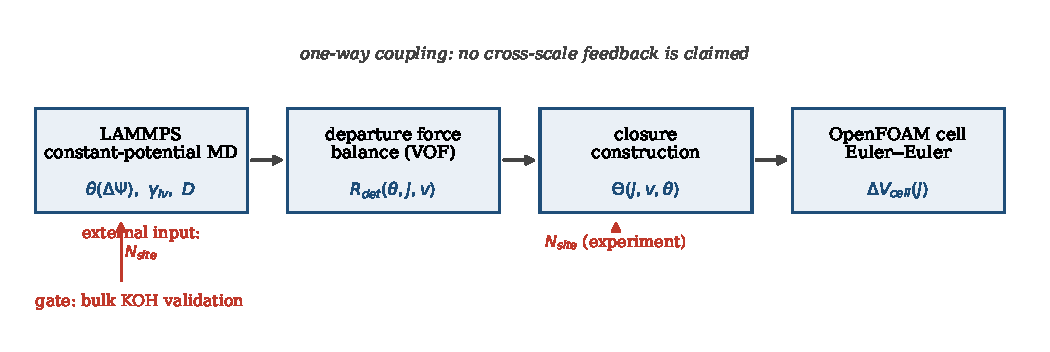
\includegraphics[width=\textwidth]{../figures/fig4_pipeline.pdf}
\caption{One-way coupling chain. Each stage passes a named quantity forward with a stated validity
range. Nucleation-site density $N_{\mathrm{site}}$ enters as an external input rather than being
derived, and the bulk-KOH validation gate precedes all interface work.}
\label{fig:pipeline}
\end{figure}

\begin{table}[htbp]\centering\small
\caption{Cross-scale coupling contract (abridged).}
\label{tab:coupling}
\begin{tabular}{@{}llll@{}}
\toprule
From $\rightarrow$ To & Quantity & Validity range & Uncertainty carried \\
\midrule
MD $\rightarrow$ bridge & $\theta(\Delta\Psi,c,T)$ & $\Delta\Psi\le\SI{1.0}{\volt}$; 20--30\,wt\%; 298--\SI{353}{\kelvin} & replica spread \\
MD $\rightarrow$ VOF & $\gamma_{lv}(c,T)$ & as above & Kirkwood--Buff block SE \\
MD $\rightarrow$ VOF/cell & $D_{\mathrm{H_2}}(c,T)$ & as above & finite-size-corrected fit SE \\
bridge $\rightarrow$ VOF & wall contact-angle BC & per case & campaign repeated at $\theta\pm\sigma_\theta$ \\
Cantera $\rightarrow$ all & $j_0(T,c)$ & tabulated, clamped at edges & mechanism uncertainty stated \\
VOF $\rightarrow$ regression & $\Theta_{\mathrm{adh}}$, $A_{\mathrm{cov,proj}}$ & $j\,10^2$--$10^4$; $v\,0$--0.2; $\theta\,30$--\ang{150} & time-averaging SE \\
regression $\rightarrow$ cell & closure $\Theta(j,v,\theta)$ & the above box $\cap$ $\Lambda>1$ & 95\,\% CI on parameters \\
\bottomrule
\end{tabular}
\end{table}

The closure implementation \textbf{raises an error rather than extrapolating} outside its validity
box. This is deliberate: the study exists because a closure was extrapolated far beyond its
validated range, and reproducing that error with a new closure would be self-defeating.

%==========================================================================
\section{Methods}\label{sec:methods}

All simulations use open-source software on a single Linux workstation (16 physical cores,
\SI{23}{\giga\byte} RAM, no GPU).

\subsection{Molecular dynamics}
\paragraph{Code and electrostatics.} LAMMPS (22 Jul 2025 stable) built from source with the
\textsc{electrode} package, MPI and FFTW3. Long-range electrostatics use
\texttt{pppm/electrode} with slab correction for the 2D-periodic geometry.

\paragraph{Constant-potential electrodes.} Electrode atoms carry Gaussian charges solved each
timestep so that every electrode atom sits at its imposed potential, via
\texttt{fix electrode/conp}:
\begin{equation}
\mathbf{A}\,\mathbf{q} = \mathbf{b}(\Psi,\{\mathbf{r}\}),\qquad \sum_i q_i = 0,\qquad
\Delta\Psi = \Psi_{\mathrm{anode}} - \Psi_{\mathrm{cathode}}
\end{equation}
The implementation was verified against the reference case distributed with the package,
reproducing published induced electrode charges to all printed digits across the full potential ramp.
In the production geometry $\sum_i q_i = 0$ holds exactly at every timestep, with induced charges
equal and opposite on the two slabs and growing as the double layer forms.

\paragraph{System and force field.} Ni(111) slabs of five layers ($a=\SI{3.524}{\angstrom}$) bound an
aqueous KOH film; water is SPC/E with SHAKE constraints. Potassium uses Joung--Cheatham parameters
optimised for SPC/E~\verifyc. The hydroxide representation is the subject of
Section~\ref{sec:ffgate} and was revised after validation.

\paragraph{Initialisation.} Lattice configurations are relaxed by a displacement-capped
\texttt{nve/limit} push under a strong Langevin thermostat rather than by energy minimisation,
because SHAKE constraints are ignored during minimisation in LAMMPS and a minimised configuration is
therefore not consistent with the constrained dynamics that follow.

\paragraph{Contact-angle protocol.} A cylindrical (quasi-2D) hydrogen bubble, periodic along its
axis, rests on the cathode. The interface is the isochore of the time-averaged density field at
$\rho = \tfrac12(\rho_l+\rho_g)$, and the angle is measured \emph{through the liquid}, matching the
continuum wall boundary condition.

\textbf{No line-tension extrapolation is performed, and none is possible in this geometry.} A
periodic cylindrical cap has straight contact lines with zero in-plane geodesic curvature, so the
modified Young relation $\cos\theta(R)=\cos\theta_\infty - \tau/(\gamma_{lv}R)$, derived for a
\emph{circular} contact line, does not apply. Cylindrical geometry is used precisely because it
\emph{suppresses} the line-tension contribution. Size dependence is instead addressed by box-size
convergence at lateral widths of 8, 12 and \SI{16}{\nano\metre} (19k, 30k and 41k atoms), required to
be invariant within replica scatter. This is a convergence check on periodic-image and opposing-wall
artefacts, not a physical extrapolation.

\paragraph{Statistics and referencing.} Each state point uses at least three independent seeds, and
reported uncertainty is the spread across replicas, because block averages from a single trajectory
are not independent realisations. The control variable is the electrode potential relative to the
potential of zero charge; the raw inter-slab potential difference is a cell voltage, not an electrode
potential. The Lippmann relation
$\cos\theta(\Delta\Psi)=\cos\theta_{\mathrm{pzc}} + C_{dl}(\Delta\Psi-\Psi_{\mathrm{pzc}})^2/(2\gamma_{lv})$
predicts a shift of roughly \ang{10}--\ang{31} for $C_{dl}=0.1$--$\SI{0.3}{\farad\per\square\metre}$
over a \SI{0.5}{\volt} excursion.

\subsection{Force-field validation gate}\label{sec:ffgate}
The molecular model is validated against bulk KOH(aq) properties \emph{before} any interface
calculation. Systems of 20 and 30\,wt\% KOH are equilibrated at 298 and \SI{333}{\kelvin} with three
seeds each; density and self-diffusivities are compared with experiment, the latter from the Einstein
relation over the linear region of the mean-squared displacement with a finite-size correction.

Pass criteria were fixed before any result was inspected: density within 3\,\%, $D(\mathrm{H_2O})$
within 30\,\%, $D(\mathrm{K^+})$ within 40\,\%. \textbf{Hydroxide diffusivity is reported but not
gated}, because a single-site classical hydroxide cannot reproduce structural (Grotthuss) diffusion
and is expected to be too slow; treating that as a force-field failure would be a category error, and
treating it as acceptable without saying so would be worse.

\subsection{Interface-resolved two-phase simulation}
OpenFOAM v2406, geometric VOF (\texttt{interIsoFoam}), with custom boundary conditions compiled
against the standard library. Wall wettability enters through
\begin{equation}
\hat{\mathbf{n}}_{\mathrm{wall}}\cdot\frac{\nabla\alpha}{|\nabla\alpha|} = \cos\theta
\label{eq:wallbc}
\end{equation}
with $\theta$ from the molecular calculation. \textbf{Equation~\eqref{eq:wallbc} is the single point
at which the molecular result enters the continuum model.}

Bubble growth is driven by dissolved-hydrogen transport with a Henry-law interfacial condition and a
Faradaic wall flux applied over the exposed area in the current-conserving form
\begin{equation}
N_{\mathrm{H_2,exposed}} = \frac{j}{2F(1-\Theta)},\qquad
\int_{\mathrm{exposed}} N_{\mathrm{H_2}}\,\mathrm{d}A = \frac{j A_{\mathrm{geom}}}{2F}
\label{eq:flux}
\end{equation}
The normalisation matters: applying $j/(2F)$ over the uncovered area instead would reduce total gas
generation to $(1-\Theta)j/(2F)$ and violate the imposed galvanostatic current, artificially
suppressing bubble growth as coverage rises. The same convention is used in the gas source term, the
electrode boundary condition and the closure.

\paragraph{Geometry.} The parametric campaign is axisymmetric, on a wedge sized to five expected
departure radii, with mesh spacing holding $\approx$25 cells per expected departure radius at each
current density (\SI{5.0}{\micro\metre} at $100\ \mathrm{A\,m^{-2}}$ down to \SI{1.5}{\micro\metre} at
$10^4\ \mathrm{A\,m^{-2}}$). This follows from measured throughput: a three-dimensional parametric
sweep at contact-line resolution would need $\sim1.6\times10^7$ cells per case against a practical
memory ceiling of $\sim5\times10^6$, and is not feasible. Two contrasting three-dimensional cases at
reduced resolution bound the effect of the axisymmetric restriction.

\paragraph{Initialisation.} Bubbles are seeded at $0.85$ of the expected departure radius, the
preceding quasi-static growth being treated analytically. The departure radius remains an
\emph{output} of Eq.~\eqref{eq:forcebal}, not an input: the seed lies well below departure so the
detachment event is predicted rather than prescribed. This is necessary because growing a bubble from
nucleation at $100\ \mathrm{A\,m^{-2}}$ requires seconds of physical time and $\sim10^7$ timesteps.

\subsection{Verification before production}
Two verification cases gate the campaign; no production case runs until both pass.
(i)~Diffusion-driven growth against the Epstein--Plesset/Scriven similarity solution
$R(t)=2\beta\sqrt{Dt}$. (ii)~Variable surface tension and the tangential Marangoni stress against an
analytic thermocapillary benchmark---this case exists because a wrongly scaled or signed
$\nabla_s\gamma$ produces a plausible-looking but meaningless regime map, and because with constant
surface tension $F_{\mathrm{Mar}}\equiv0$ and the regime bound would be untestable by construction.
Mesh independence is established at three refinement levels with Richardson extrapolation and a
reported grid convergence index.

\subsection{Construction of the coverage closure}\label{sec:closure}
Coverage is \emph{constructed}, not regressed directly from a single-bubble calculation:
\begin{equation}
\Theta = N_{\mathrm{site}}\cdot A_{\mathrm{footprint}}(\theta,R_{\mathrm{det}})
\cdot f_{\mathrm{residence}}(j,v,\theta)\cdot f_{\mathrm{overlap}}
\label{eq:cov}
\end{equation}
The resolved simulations supply $A_{\mathrm{footprint}}=\pi R_{\mathrm{det}}^2\sin^2\theta$, the
departure radius $R_{\mathrm{det}}(\theta,j,v)$ from Eq.~\eqref{eq:forcebal}, and the residence time
per cycle over several stationary departure events. \textbf{The active nucleation-site density
$N_{\mathrm{site}}$ is an explicit external input}, taken from experiment and stated with its source
and uncertainty; it is dominated by sub-surface cavity geometry and surface finish, which molecular
dynamics of a flat single-crystal slab cannot supply.

The functional form is specified before fitting so it cannot be reverse-engineered from the data:
\begin{equation}
\Theta(j,v,\theta) = C\left(\frac{j}{j_{\mathrm{ref}}}\right)^{a} g(\theta)\,h(v),
\qquad g(\theta)=\left[\frac{1-\cos\theta}{1-\cos\theta_{\mathrm{ref}}}\right]^{b}
\end{equation}
with $h(v)$ retained in the form of Eq.~\eqref{eq:vogtflow} so the flow dependence is directly
comparable with the legacy correlation. Twenty per cent of the campaign is held out as a test set,
and fitted parameters are reported with 95\,\% confidence intervals and held-out RMSE.

\textbf{Two coverage measurands are extracted, not one}: the adhering-bubble surface coverage
$\Theta_{\mathrm{adh}}$, which screens catalytic area, and a synthetic projected coverage
$A_{\mathrm{cov,proj}}$ obtained by rendering the resolved interface as a top-view optical
measurement would see it. These differ by $\sin^2\theta$ for a spherical cap even before detached
bubbles in the field of view are considered---a factor of 4 at \ang{30}---and reporting both is what
allows the apparent disagreement between optical and electrochemical coverage measurements to be
addressed quantitatively rather than asserted away.

\subsection{Cell-scale model and quality control}
The closure is implemented in an Euler--Euler two-fluid model
(\texttt{reactingMultiphaseEulerFoam}) with named drag, lift, wall-lubrication and
turbulent-dispersion closures, charge transport by Eq.~\eqref{eq:brugg}, and the electrode boundary
condition carrying $\Theta$ into Eq.~\eqref{eq:bv}. Exchange current density is supplied by a Cantera
surface-kinetics evaluation, pre-tabulated and interpolated at run time. The reported quantity is
$\Delta V_{\mathrm{cell}}(j) = U_{\mathrm{cell}}[\Theta_{\mathrm{Vogt}}]
- U_{\mathrm{cell}}[\Theta_{\mathrm{this\ work}}]$, evaluated only inside the closure's validity box.

Every run batch is checked automatically for mass and charge conservation, Courant and residual
convergence, boundedness of $\alpha$ and $\Theta$, monotonicity of the polarisation curve, MD energy
drift, the presence of replica-based uncertainties on every reported mean, and the adhering/dispersed
gas transfer. A check failing twice freezes that branch pending review rather than being retried.

%==========================================================================
\section{Results}\label{sec:results}

\subsection{Force-field validation: the gate rejected the initial model}\label{sec:res-gate}

The hydroxide ion was initially represented as a single Lennard-Jones site carrying unit negative
charge with parameters taken identical to SPC/E oxygen
($\sigma=\SI{3.166}{\angstrom}$, $\varepsilon=\SI{0.1553}{kcal\per\mole}$), following practice
reported for hydroxide in SPC/E-based simulations. \textbf{This model failed the pre-registered
density gate at every state point} (Fig.~\ref{fig:gate}, Table~\ref{tab:gate}).

\begin{table}[htbp]\centering\small
\caption{Bulk KOH(aq) validation against experiment. Three independent seeds per state point;
uncertainty is the replica spread. The pre-registered tolerance is 3\,\%.}
\label{tab:gate}
\begin{tabular}{@{}lccccc@{}}
\toprule
System & $\rho_{\mathrm{sim}}$ (\si{\gram\per\cubic\centi\metre}) & $\rho_{\mathrm{exp}}$ &
Error & $D_{\mathrm{H_2O}}$ (\si{\metre\squared\per\second}) & Verdict \\
\midrule
20\,wt\%, \SI{298}{\kelvin} & $1.2672\pm0.0020$ & 1.188 & $+6.67\,\%$ & $8.79\times10^{-10}$ & FAIL \\
20\,wt\%, \SI{333}{\kelvin} & $1.2367\pm0.0021$ & 1.163 & $+6.33\,\%$ & $1.81\times10^{-9}$  & FAIL \\
30\,wt\%, \SI{298}{\kelvin} & $1.4081\pm0.0048$ & 1.290 & $+9.16\,\%$ & $3.28\times10^{-10}$ & FAIL \\
30\,wt\%, \SI{333}{\kelvin} & $1.3817\pm0.0008$ & 1.265 & $+9.23\,\%$ & $8.75\times10^{-10}$ & FAIL \\
\bottomrule
\end{tabular}
\end{table}

\begin{figure}[htbp]\centering
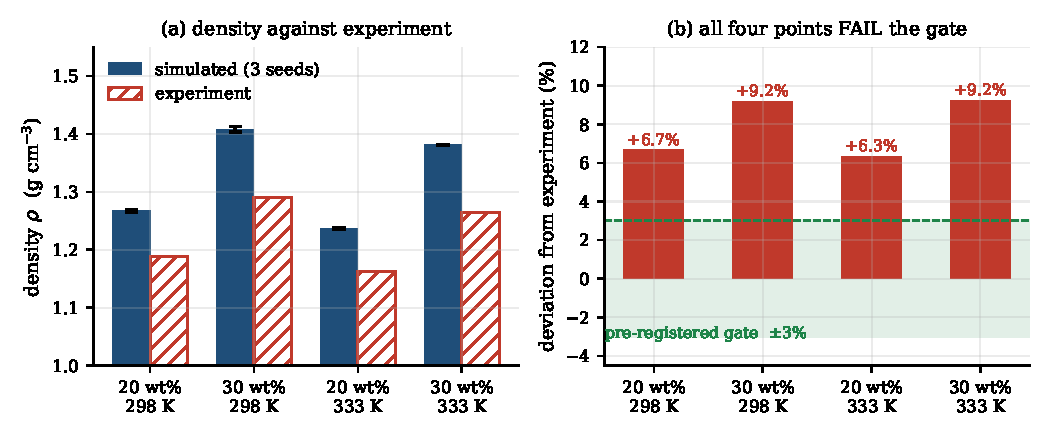
\includegraphics[width=\textwidth]{../figures/fig1_density_gate.pdf}
\caption{Bulk KOH density against experiment. (a)~Simulated density (three seeds, error bars are
replica spread) against experimental values. (b)~Deviation from experiment; the shaded band is the
pre-registered $\pm3\,\%$ tolerance. All four state points fail, and the error grows with electrolyte
concentration.}
\label{fig:gate}
\end{figure}

Three features make the failure diagnostic rather than merely disqualifying.

\textbf{It is systematic, not statistical.} Replica scatter is
0.002--\SI{0.005}{\gram\per\cubic\centi\metre} against a discrepancy of
0.08--\SI{0.12}{\gram\per\cubic\centi\metre}: the error exceeds the seed-to-seed spread by a factor
of 20--60.

\textbf{It scales with electrolyte concentration}, from $+6.5\,\%$ at 20\,wt\% to $+9.2\,\%$ at
30\,wt\%. An error that grows with ion content implicates the ion parameters rather than the water
model.

\textbf{Transport corroborates over-structuring.} The water self-diffusivity
(Fig.~\ref{fig:transport}) falls to $3.28\times10^{-10}\ \mathrm{m^2\,s^{-1}}$ at 30\,wt\% and
\SI{298}{\kelvin}, roughly seven-fold below neat water, a stronger suppression than concentrated KOH
exhibits experimentally. The electrolyte is simultaneously too dense and too strongly bound,
consistent with excessive ion--water attraction.

\begin{figure}[htbp]\centering
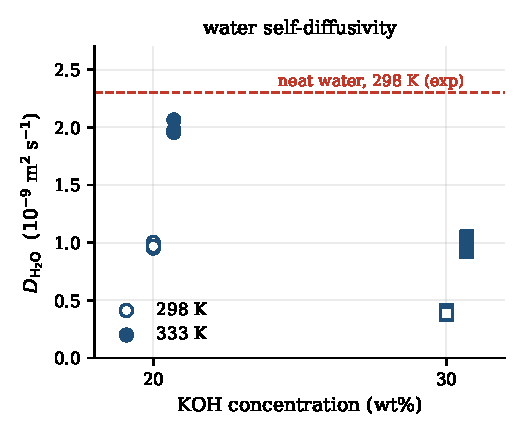
\includegraphics[width=0.52\textwidth]{../figures/fig2_transport.pdf}
\caption{Water self-diffusivity from the Einstein relation. Open symbols \SI{298}{\kelvin}, filled
\SI{333}{\kelvin}; each point is one seed. The dashed line is the experimental value for neat water
at \SI{298}{\kelvin}. The suppression at 30\,wt\% is substantially stronger than experiment
indicates, corroborating the over-structuring implied by the density error.}
\label{fig:transport}
\end{figure}

The gate therefore performed its intended function: it rejected the model \emph{before} the
contact-angle campaign was committed, which would otherwise have produced a confidently wrong
wettability and propagated it silently into the closure, the cell model, and the headline result.
\pending{Revised hydroxide parametrisation and re-validation. The tolerance was not widened to
accommodate the failure.}

\subsection{Remaining results}
\pending{Contact angle under electrode polarisation, and box convergence.}\\
\pending{Verification cases (Scriven growth; thermocapillary benchmark).}\\
\pending{Departure radius and the force balance.}\\
\pending{The regime bound $\Lambda(j,v)$.}\\
\pending{The derived closure and its validity box.}\\
\pending{Adhering versus projected coverage.}\\
\pending{Cell polarisation: legacy versus derived closure.}

%==========================================================================
\section{Limitations}
Several limitations are structural rather than incidental.

\textbf{The molecular model is chemically inert.} SPC/E water with classical ions on a clean Ni(111)
surface cannot represent nickel oxidation, hydroxylation, specific adsorption or bond formation.
\texttt{fix electrode/conp} makes the metal \emph{charge} responsive; it does not make the interface
\emph{chemically} reactive. The reported angle is the electrostatic double-layer contribution to
potential-dependent wettability on an idealised surface, not a prediction for an operating electrode.

\textbf{Hydroxide transport is structurally limited.} A single-site classical $\mathrm{OH^-}$ cannot
carry Grotthuss transport; its diffusivity is reported but not used as a continuum input, and
electrolyte transport properties are taken from experiment.

\textbf{Molecular dynamics supplies an equilibrium angle, not hysteresis.} The continuum model
requires advancing and receding angles under flow; these come from measured data with the molecular
calculation informing the equilibrium centre.

\textbf{Nucleation-site density is an input, not a result}, so the closure's wettability and flow
dependence are derived while its absolute level inherits the uncertainty of the declared
$N_{\mathrm{site}}$.

\textbf{The parametric campaign is axisymmetric}, so lateral motion, sliding and coalescence are
absent, and shear-induced asymmetric contact-line depinning---expected to reduce departure radius in
cross-flow---is suppressed. Two contrasting three-dimensional cases bound this; they do not eliminate
it.

\textbf{The Bruggeman exponent is not validated for this system} and is carried as a sensitivity
parameter. \textbf{The regime bound is computed for clean electrolyte} without surfactants, for a
single bubble, and is scoped accordingly.

%==========================================================================
\section*{Data availability}
All simulation inputs, analysis scripts, verification cases and the closure implementation are
available in the accompanying repository. The corpus analysis underlying Section~\ref{sec:intro} is
identified by hash \texttt{9dd4b795a80ec687}. \pending{Repository DOI to be minted on submission.}

%==========================================================================
\begin{thebibliography}{99}\small
\bibitem{vogt2005} H. Vogt, R.J. Balzer, The bubble coverage of gas-evolving electrodes in stagnant
electrolytes, \emph{Electrochim. Acta} (2005). \url{https://doi.org/10.1016/j.electacta.2004.09.025}
\bibitem{eigeldinger2000} J. Eigeldinger, H. Vogt, The bubble coverage of gas-evolving electrodes in
a flowing electrolyte, \emph{Electrochim. Acta} \textbf{45} (2000) 4449--4456. (No DOI is printed in
the source; volume and pages as printed.)
\bibitem{jacobsen2025} A.N. Jacobsen, E. Mahravan, M.V. Kragh-Schwarz, J. Catalano, P. Fooroghi,
Multiphysics simulations of alkaline water electrolyzer cells --- a sensitivity study on the effect
of two-phase flow modeling, \emph{Electrochim. Acta} (2025).
\url{https://doi.org/10.1016/j.electacta.2025.147148}
\bibitem{li2024} J. Li, H. Liang, M.A. Rehan, G. Li, Numerical simulation and analysis of a two-phase
flow model considering bubble coverage for alkaline electrolytic water, \emph{Appl. Therm. Eng.}
\textbf{245} (2024) 122890. \url{https://doi.org/10.1016/j.applthermaleng.2024.122890}
\bibitem{moyo2026} O. Moyo, H. Sun, J. Yang, X. Xu, Z. Shao, Gas bubble formation, effect on
electrode performance, and management in water electrolysis, \emph{Nano Energy} (2026).
\url{https://doi.org/10.1016/j.nanoen.2026.112024}
\bibitem{zhang2024sm} H. Zhang, Y. Ma, M. Huang, G. Mutschke, X. Zhang, Solutal Marangoni force
controls lateral motion of electrolytic gas bubbles, \emph{Soft Matter} \textbf{20} (2024)
3097--3106. \url{https://doi.org/10.1039/D3SM01646C}
\bibitem{kitajima2024} D. Kitajima, R. Misumi, Y. Kuroda, S. Mitsushima, Relationship between bubble
generation behavior and hydrogen evolution reaction performance at high current densities during
alkaline water electrolysis, \emph{Electrochim. Acta} \textbf{502} (2024) 144772.
\url{https://doi.org/10.1016/j.electacta.2024.144772}
\bibitem{hammons2024} J. Hammons et al., Nanobubble formation and coverage during high current
density alkaline water electrolysis, \emph{Nano Lett.} (2024).
\url{https://doi.org/10.1021/acs.nanolett.4c03657} \verifyc\ author list to be completed
\bibitem{rox2022} H. Rox, A. Bashkatov, X. Yang, S. Loos, G. Mutschke, G. Gerbeth, K. Eckert, Bubble
size distribution and electrode coverage at porous nickel electrodes in a novel 3-electrode
flow-through cell, arXiv:2209.11550 (2022). \verifyc\ check for journal version
\bibitem{zarghami2020} A. Zarghami, N.G. Deen, A.W. Vreman, CFD modeling of multiphase flow in an
alkaline water electrolyzer, \emph{Chem. Eng. Sci.} (2020).
\url{https://doi.org/10.1016/j.ces.2020.115926}
\bibitem{kanemoto2025} R. Kanemoto, T. Araki, R. Misumi, S. Mitsushima, Numerical modeling of
two-phase flow considering multiple bubble sizes in an alkaline water electrolyzer,
\emph{Chem. Eng. Sci.} \textbf{304} (2025) 120986. \url{https://doi.org/10.1016/j.ces.2024.120986}
\bibitem{andersson2023} L. Andersson, C. Zhang, Molecular dynamics simulations of metal-electrolyte
interfaces under potential control, \emph{Curr. Opin. Electrochem.} (2023).
\url{https://doi.org/10.1016/j.coelec.2023.101407}
\bibitem{zhang2024cpc} S. Zhang, S. Hess, H. Marschall, U. Reimer, S. Beale, et al., openFuelCell2: a
new computational tool for fuel cells, electrolyzers, and other electrochemical devices and
processes, \emph{Comput. Phys. Commun.} \textbf{298} (2024) 109092.
\url{https://doi.org/10.1016/j.cpc.2024.109092}
\bibitem{han2025} Y. Han, M. Huang, K. Eckert, G. Mutschke, Numerical simulation of
oversaturation-driven bubble growth on solid surfaces with dynamic wetting,
\emph{Int. J. Multiphase Flow} (2025). \url{https://doi.org/10.1016/j.ijmultiphaseflow.2025.105343}
\bibitem{vacha2021} K.J. Vachaparambil, K.E. Einarsrud, Numerical simulation of continuum scale
electrochemical hydrogen bubble evolution, \emph{Appl. Math. Model.} \textbf{98} (2021) 343--377.
\url{https://doi.org/10.1016/j.apm.2021.05.007}
\bibitem{spce} H.J.C. Berendsen, J.R. Grigera, T.P. Straatsma, The missing term in effective pair
potentials, \emph{J. Phys. Chem.} \textbf{91} (1987) 6269--6271. \verifyc
\bibitem{joung2008} I.S. Joung, T.E. Cheatham III, Determination of alkali and halide monovalent ion
parameters for use in explicitly solvated biomolecular simulations, \emph{J. Phys. Chem. B}
\textbf{112} (2008). \verifyc\ pages to be confirmed
\bibitem{riegel} Riegel et al., local gas-fraction measurements in an alkaline electrolyser
(1997/1998), as reported in refs~\cite{zarghami2020} and~\cite{li2024}. \verifyc\ primary reference
to be obtained
\end{thebibliography}

\end{document}
